% Please do not change the document class
\documentclass{scrartcl}

% Please do not change these packages
\usepackage[hidelinks]{hyperref}
\usepackage[none]{hyphenat}
\usepackage{setspace}
\doublespace

% You may add additional packages here
\usepackage{amsmath}
\usepackage{graphicx}

% Please include a clear, concise, and descriptive title
\title{Research Journal - Brain controlled games via brain-computer interfaces}

% Please do not change the subtitle
\subtitle{COMP160 - Software Engineering Essay}

% Please put your student number in the author field
\author{1603748}

\begin{document}

\maketitle

\abstract{abstract}

\section*{Introduction}
A brain-computer interface (BCI), also known as a brain-machine interface (BMI), is a system that enables users to interact with external devices based solely on changes in brain activity \cite{Checkers}. This is achieved through the use of electrical signals that occur in the brain after estimate a human intention \cite{SharedRacing}. BCI research was originally focused on helping patients who suffer from amyotrophic
lateral sclerosis (ALS) and motor neuron disease. However, recently more work has also been done to create BCI technology for gaming with the intention of providing concentration improvement and entertainment to the general public \cite{SharedRacing},\cite{Spacecraft}. In this research journal I look at various different BCI-controlled games that use different BCI methods and sensors, particularly steady-state visually evoked potential (SSVEP) \cite{Checkers}, \cite{GamingSystem}, \cite{Spacecraft} and electroencephalography (EEG) \cite{GamingControlling}, \cite{SharedRacing}, \cite{AndroidRacing} . I will compare multiple different ways to use BCI in games, including using wet or dry electrodes, invasive/nonivasive and the way the users interact with the games. The two most common types of BCI systems used with games are steady steady-state visually evoked potentials (SSVEPs) and electroencephalography (EEG)

\section*{EEG-based BCIs}
The use of electroencephalographic (EEG) signals has become a very common approach to BCI because of their usability and strong reliability \cite{GamingControlling}.

\subsection*{Gaming controlling via brain-computer interface using multiple physiological signals}
Shi-An Chen et als study \cite{GamingControlling} proposes a wireless EEG and EOG (Electrooculography) BCI system which was tested with a simple baseball game. Their system was highly accurate and the users found it easy and fun to play the baseball game. The paper described a single processing method, which uses a wireless EEG-based BCI system designed to be worn near forehead that can detect both EEG and EOG signals, for detecting eye movements to have 9 direction controls
(via EOG) and one action of execution (via EEG) \cite{GamingControlling}. They concluded that ``compared with other eye movement detection methods, no more electrodes are needed in our system to extract EEG signals" \cite{GamingControlling}. They found that other EEG-based BCIs are too large and uncomfortable which was inconvenient for users. They made developing a portable device that was smaller than other EEG-based BCIs and comfort an important goal. They also decided to to incorporate wireless technology as enable use of the system in daily life, wireless transmission is also more convenient for transmitting EEG and EOG data than other data transmission methods. 

\subsection*{A brain-computer interface for shared vehicle control on TORCS car racing game}
\cite{SharedRacing} D. Kim and S. B. Cho developed an EEG-based BCI system that controls a 3D racing game simulator know as TORCS. They used a shared vehicle control system using EEG to provide faster intention cognition response than an electromyography (EMG) system. This was used because ``In the racing game or First-person shooter (FPS) games, fast intention cognition is important. In the case of racing games, in order to overtake the car ahead, the handle must be controlled quickly'' \cite{SharedRacing}. The sensorimotor rhythm (SMR) method was used to construct the virtual car racing simulator. SMR is used as a command paradigm to extract EEG signals corresponding to the players right hand, left hand and both hands. Two experiments were used in this paper, one solve the EEG binary classification problem and the other was for the classification of different hand EEG signals. The BCI system used in this paper has four sections, preprocessing, feature extraction, classification, and control session as shown in figure 1 \cite{SharedRacing}.

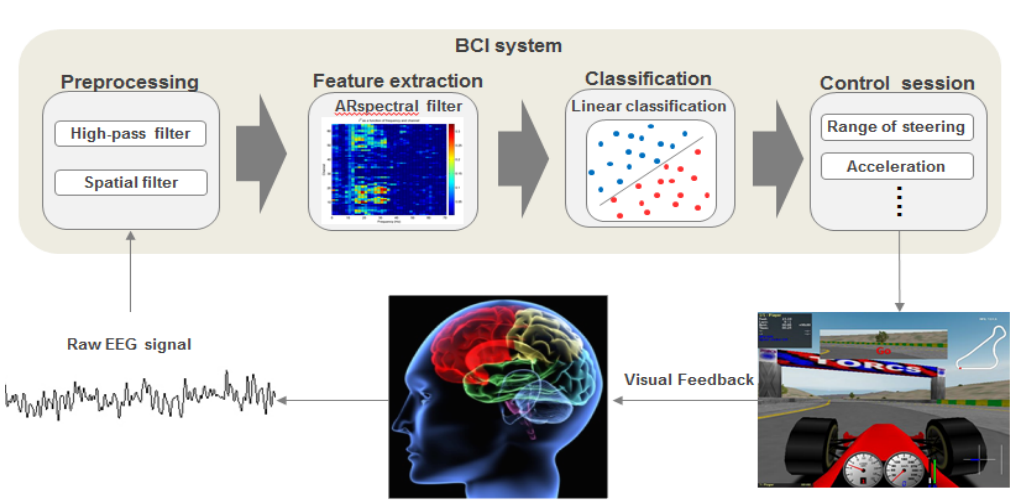
\includegraphics[width=\textwidth]{TORCS_BCI}
Figure 1. The shared vehicle control system configuration \cite{SharedRacing}

In the pre-processing, spacial filters are used to increase the accuracy of the car driving and the high-pass filter cuts off frequency less than 0.1 Hz. Feature extraction removes redundant information and extracts all the interesting and useful information. This information then goes through a linear classification system then goes to the control session which controls the range of steering and acceleration of the car in the game. 


\subsection*{Development of a mind-controlled Android racing game using a brain computer interface}
``Recently, with the development of BCI, several research institutions and organizations have developed some games that are interacted with BCI to enrich user's experience. However, most of these games are only used in computers and just focus on the realization of direction strategies'' \cite{AndroidRacing}. G. Wu et al presented a racing game that is on the android system and uses a commercially available BCI (mindset) to enable the user to control the game through their neural mind states. They wanted to create a game that doesn't just focus on movement direction control strategies like many other BCI-controlled games \cite{GamingControlling}, instead they used the user's mental state data. BCIs can be either invasive or noninvasive. Invasive BCI systems require the user to have sensors implanted into their brain, while noninvasive sensors are external and are just touching the skin. Noninvasive BCIs are much more common than invasive because they are much more convenient, however they have a much weaker bioelectricity signal. In this paper an invasive BCI was used for convenience so it could be used in daily life.

\section*{SSVEP-based BCIs}
steady-state visually evoked potential (SSVEP) based BCI systems for games are becoming very common. They work by measuring when the user's brain is stimulated by something, usually a flickering light. ``SSVEPs are elicited when a user focuses his attention on a flickering visual stimulus appearing at a frequency between 1-100Hz'' \cite{Checkers}

\subsection*{Playing checkers with your mind: An interactive multiplayer hardware game platform for brain-computer interfaces}
There has been lots of software-based BCI games produced which use a computer screen, but there are very few hardware based games that use BCIs. A. Akhtar et al \cite{Checkers} developed an interactive multiplayer hardware game platform with an SSVEP-based BCI. They chose to use SSVEP is because they require very little pre-run classifier training and also have a higher transfer rates than P300-based BPIs such as the P300-based Tetris \cite{TetrisP300} or motor imagery based systems. 

\subsection*{Design a brain computer interface gaming system using steady-state visual evoked potential}
Many BCI systems adopt wet-type electrodes which require preparation before the user can interact with the computer. L. Po-Lei et al \cite{GamingSystem} demonstrated the use of dry electrodes to control a two-selection claw gaming system. ``These wet-type electrodes are not convenient for use. requires a lousy preparation process and the refill of electrolyte after using one or two hours''\cite{GamingSystem}. An example of a BCI system that uses these wet-type electrodes is the SSVEP-based spacecraft game \cite{Spacecraft}. They wanted to use dry electrodes because it is more comfortable and convenient for users since no preparation is needed. 

\subsection*{A spacecraft game controlled with a brain-computer interface using SSVEP with phase tagging}
R. Parafita et al \cite{Spacecraft} presented a SSVEP-based BCI spacecraft game in their paper. The game displays two flickering stimuli on the left and right of the screen which the user uses to move the spacecraft left or right. The stimuli used in this game is within a 3-5 Hz range which is an advantage over over SSVEP approaches as it causes less eye strain. One interesting point they brought up was that BCIs rely on the user paying attention, so games are an obvious choice for this as they easily capture people's attention.  

\section*{Conclusion}
I have summarised a number of different uses of BCI technology in games. I personally prefer the EEG-based systems as they seem more controlled solely by you rather than by stimuli conveniently placed in the game. However SSVEP-based systems tend to be more accurate, the spacecraft game \cite{Spacecraft} had 95 percent accuracy.

From what I have learnt, BCI games can be very beneficial, not just for handicapped patients, but also for people who want to recover from stroke incidents or brain injuries. This is because they can be used as a neurorehabilitation tool \cite{Spacecraft}. In addition BCI games could be used by the general public to provide concentration improvement as well as entertainment of course.

\bibliographystyle{IEEEtran}
\bibliography{references}

\end{document}
